\newpage
\section{Билет 20. Задача об изгибе балки.}

Рассмотрим упругую цилиндрическую балку произвольного поперечного сечения.

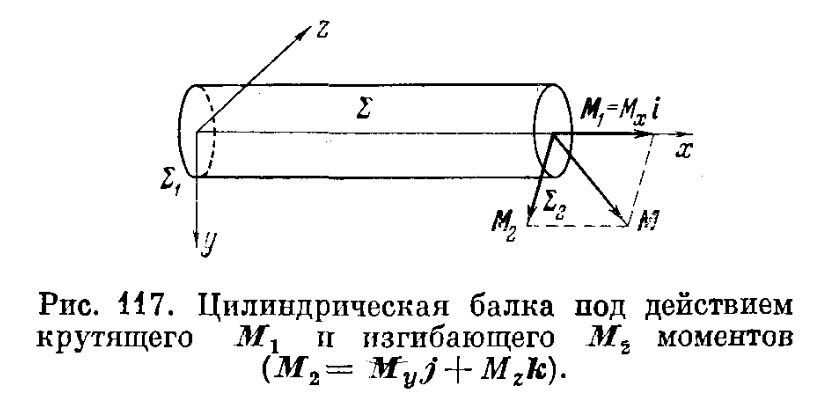
\includegraphics[scale=0.5]{20/t21_1.jpg}


\noindent Боковая поверхность балки $\Sigma$ не нагружена $\vec{p^n} = 0$.

\noindent На торце $\Sigma_2$ $\vec{p^n} \neq 0$, причем
$$\int_{\Sigma_2} {\vec{p^n} d{\sigma}} = 0,
\int_{\Sigma_2} (\vec{r} \times \vec{p^n}) d{\sigma} = \vec{M} \neq 0,$$

\noindent т.е. на торце $\Sigma_2$ балки действует пары сил с общим моментом $\vec{M}$. Балка по условию находиться в равновесии, поэтому на торце $\Sigma_1$

$$\int_{\Sigma_1} {\vec{p^n} d{\sigma}} = 0,
\int_{\Sigma_1} (\vec{r} \times \vec{p^n}) d{\sigma} = -\vec{M}$$

\noindent В общем случае момент $\vec{M}$ может иметь произвольное направление.

Выберем правую декартову систему координат $x$, $y$, $z$ так, чтобы ось $x$ была направлена по оси балки и проходила через центры тяжести поперечных сечений, а $y$, $z$ направлены по главным осям инерции поперечного сечения.

\noindent Тогда момент действующий на торце $\Sigma_2$ разложиться на три составляющие $\vec{M} = (M_x,M_y,M_z)$. Под действием $M_x$ балка будет закручиваться, а под действием моментов $M_y$, $M_z$ - изгибаться.

В силу линейности задачи общее решение получается как сумма решений трех задач: задачи о кручении под действием момента $M_x$ и двух задач об изгибе балки под действием моментов $M_y$ и $M_z$. Последние две задачи решаются аналогично.

Чистый изгиб балки $\vec{M} = (0,0,M_z)$


Распределение напряжений на торце $\Sigma_2$.
(Цитата лектора : "Угадываем решение") $\vec{p^n} = p_{11}\vec{e^1}$, $p_{11} = - \alpha y$. Проверим, что это решение на торцах удовлетворяет задаче.

Главный вектор: $ \int_{\Sigma_2} {\vec{p^n} d{\sigma}} = -\alpha \vec{e^1} \int_{\Sigma_2} {y d{\sigma}} = 0$, так как ось $x$ проходит через центр тяжести поперечного сечения.

$$ M_x = \int_{\Sigma_2} {(\vec{r} \times \vec{p^n})_x d{\sigma}} = 0,$$
\noindent так как $\vec{p^n}$ параллельно оси $x$,

$$ M_y = \int_{\Sigma_2} {(\vec{r} \times \vec{p^n})_y d{\sigma}} = \alpha \int_{\Sigma_2} {yz d{\sigma}} = 0,$$
\noindent так как оси $y$ и $z$ совпадают с главными осями инерции поперечного сечения,

$$ M = M_z = \int_{\Sigma_2} {(\vec{r} \times \vec{p^n})_z d{\sigma}} = \alpha \int_{\Sigma_2} {y^2 d{\sigma}} = \alpha J,$$
\noindent где J - момент инерции поперечного сечения относительно оси $z$. Решение удовлетворяет задаче, также найден коэффициент $\alpha$.

$$ \alpha = \frac{M}{J} $$

на другом торце аналогично, поверхностные силы распределены по закону $(\vec{p^n})_{\Sigma_1} = - (\vec{p^n})_{\Sigma_2}$

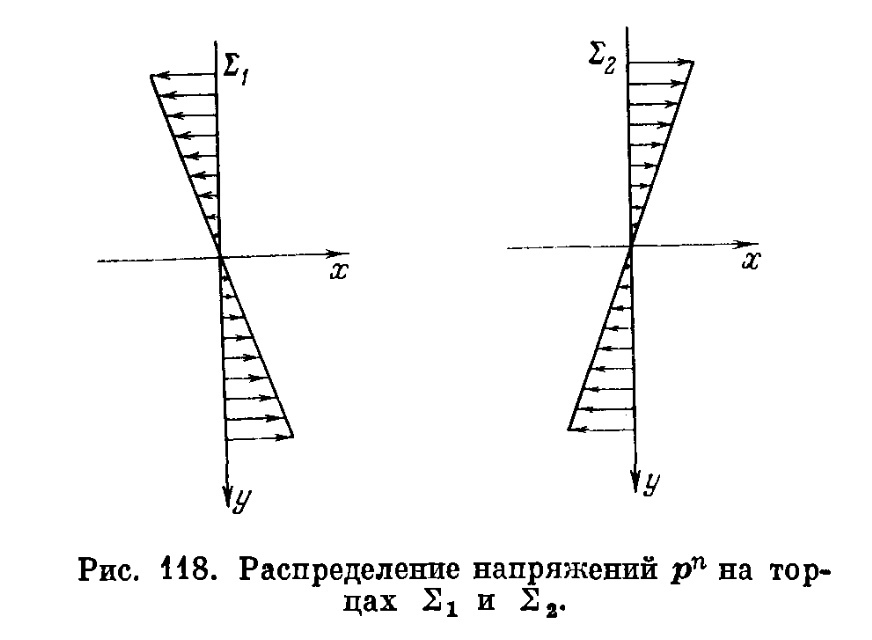
\includegraphics[scale=0.5]{20/t21_2.jpg}

Из принципа Сен-Венана следует, что полученное решение будет справедливо в части балки, достаточно удаленной от её торцов.

\noindent Тогда тензор напряжений во всех точках балки имеет вид:

\begin{equation*}
||p_{ij}|| = \left(
\begin{array}{ccc}
-\frac{M}{J}y & 0 & 0 \\
0 & 0 & 0 \\
0 & 0 & 0 \\
\end{array}
\right)
\end{equation*}

Закон Гука
$$ \varepsilon_{ij} = \frac{1}{E} \left[ (1+\sigma)p_{ij} - \sigma \mathfrak{P} g_{ij} \right] + \alpha (T-T_0)g_{ij} ,$$
где $\mathfrak{P}$ - первый инвариант тензора напряжений.

Примем, что температура во всех точках балки одинакова. Тогда по закону Гука можно вычислить компоненты тензора деформаций

\begin{equation}
\begin{array}{cc}
\varepsilon_{11} = -\frac{My}{EJ} = \frac{\partial w_1}{\partial x} & \varepsilon_{22} = \frac{\sigma My}{EJ} = \frac{\partial w_2}{\partial y} \\
\varepsilon_{33} = \frac{\sigma My}{EJ} = \frac{\partial w_3}{\partial z} & \varepsilon_{12} = \varepsilon_{23} = \varepsilon_{13} = 0
\end{array}
\end{equation}

Отсюда видно, что при чистом изгибе элементы балки, совпадающие с осью $x$, не испытывают удлинения, ни сжатия. Элементы, параллельные оси $x$, при $y>0$ сжимаются, а при $y<0$ растягиваются.

Из (1) можно найти вектор перемещения

\begin{equation}
\begin{array}{cc}
w_1 =& - \frac{Myx}{EJ} \\
w_2 =& \frac{M}{2EJ}[x^2 + \sigma (y^2 - z^2)] \\
w_3 =& \frac{\sigma Myz}{EJ}
\end{array}
\end{equation}


Любая точка балки $(x_0, y_0, z_0)$ переходит в точку с координатами $(x, y, z)$ по формулам

\begin{equation}
\begin{array}{cc}
x =& x_0 + w_1 = x_0 - \frac{My_0x_0}{EJ} \\
y =& y_0 + w_2 = y_0 + \frac{M}{2EJ}[x_0^2 + \sigma (y_0^2 - z_0^2)] \\
z =& z_0 + w_3 = z_0 + \frac{\sigma My_0z_0}{EJ}\\
\end{array}
\end{equation}

Тогда уравнение изогнутой оси балки $(y_0 = z_0 = 0)$ имеет вид
$$ y = \frac{M}{2EJ}x^2 $$

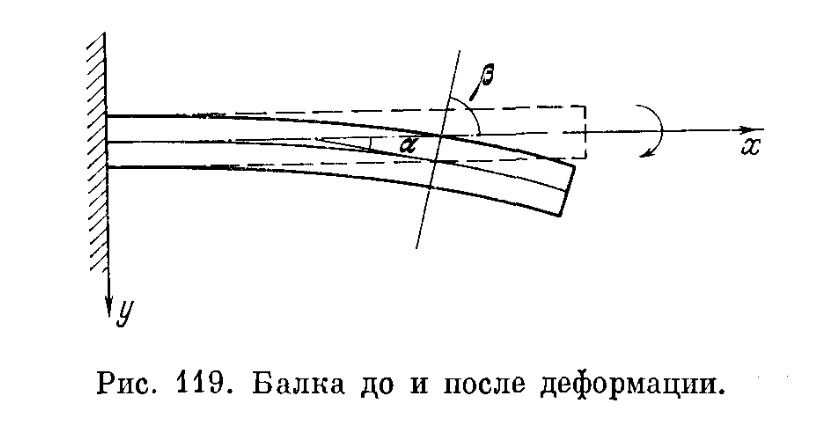
\includegraphics[scale=0.5]{20/t21_3.jpg}
